% Benötigt: \usepackage{booktabs,array}
% ENTWURF: Struktur, Tabellenvorlagen und Text sind fertig; Werte in [eckigen Klammern] kommen aus den Messläufen.
% Reproduktion: `python main.py` (Batch über ProoVer2026), `python -m src.scoring.score_proofs`, tests/ für Mutationen. Kommandos und Commit-Hash im Anhang angeben.
% Vorbedingung: Verdikt-Politik (unknown -> uncertain) und shortcut_enabled-Pfad im Code bereinigen, bevor gemessen wird (siehe Implementation, CODE-Kommentare).

\section{Evaluation}
\label{sec:evaluation}

This chapter evaluates the verifier against the research questions of Section~\ref{subsec:rq}.
Section~\ref{subsec:eval-setup} describes the benchmarks, the metrics, and the experimental setup.
Section~\ref{subsec:eval-correctness} reports correctness and score, Section~\ref{subsec:eval-coverage} the coverage of the inference rules (RQ1), and Section~\ref{subsec:eval-modularity} the properties of the architecture (RQ2).
Sections~\ref{subsec:eval-runtime} to~\ref{subsec:eval-ablation} report run time, robustness, and ablations (RQ3), and Sections~\ref{subsec:eval-errors} and~\ref{subsec:eval-threats} analyze the remaining errors and the threats to validity.

\subsection{Setup}
\label{subsec:eval-setup}

\paragraph{Benchmarks.}
The evaluation uses two proof sets.
The \emph{ProoVer set} consists of the 100 proofs \texttt{PRV000+1.s} to \texttt{PRV099+1.s} of the ProoVer 2026 benchmark, of which 47 are valid and 53 contain a deliberate error.
The \emph{TST set} consists of 76 proofs written for this thesis to test individual checks.
It is organized in six groups (Table~\ref{tab:eval-tst}); each proof has an expected result of \emph{correct} or \emph{incorrect}, and one proof is marked as an edge case whose expected result is open (inconsistent axioms, \texttt{cp03}).
The expected results of the ProoVer set were [taken from the organizers / determined by manual analysis; TODO: state the source].

\begin{table}[t]
\centering
\small
\caption{Groups of the TST set.}
\label{tab:eval-tst}
\begin{tabular}{@{}l r p{0.58\linewidth}@{}}
\toprule
Group & Proofs & Purpose \\
\midrule
\texttt{ax} & 11 & Provenance: modified, renamed, or re-roled axioms and conjectures, missing \texttt{file} directive \\
\texttt{c}  & 13 & Correct proofs with edge cases: Skolemization, renamed steps, unordered steps, nested quantifiers \\
\texttt{cp} & 3  & Conjecture used as premise, inconsistent axioms \\
\texttt{nc} & 11 & Negated conjecture: wrong status, parent, rule, role, or formula; missing or duplicated \\
\texttt{sk} & 25 & Skolemization: arity, scope, freshness, polarity, wrong result, wrong number of parents or symbols \\
\texttt{st} & 13 & Structure: no \texttt{\$false}, invalid \texttt{thm} step, cycles, undefined premises, unknown status \\
\bottomrule
\end{tabular}
\end{table}

\paragraph{Metrics.}
The primary metric is the total score under the ProoVer 2026 scheme (Section~\ref{subsec:req-scoring}): $+1$ for a correctly accepted valid proof, $+2$ for a correctly rejected invalid proof, $0$ for abstention, $-1$ for a wrongly rejected valid proof, and $-10$ for a wrongly accepted invalid proof.
In addition we report the verdict matrix (Table~\ref{tab:eval-matrix}), the number of wrong acceptances separately, the run time per proof (wall-clock and CPU), the share of steps that are decided internally, and the peak memory.

\paragraph{Environment.}
All measurements were made on [CPU, number of cores, RAM, operating system] with Python~[3.12.x], \texttt{lark}~[version], and Vampire~[version] as external prover, with the time limit of 30\,s per proof.
Each proof was checked in a fresh worker process.
Run times are medians of [5] repetitions after one warm-up run; the first run of the Lark parser builds its cached tables.
The exact commit of the verifier is [hash].

\subsection{Correctness and Score}
\label{subsec:eval-correctness}

Table~\ref{tab:eval-matrix} shows the verdicts of the verifier against the expected results.
The verifier accepts [X] of the 47 valid proofs of the ProoVer set, rejects [Y] of the 53 invalid proofs, abstains on [Z] proofs (of which [T] are timeouts), and wrongly accepts [W] proofs.
This results in a total score of [S] of a maximum of $47 + 2\cdot 53 = 153$ points.
% TODO: Falls das Ergebnis mit offiziellen ProoVer-Ergebnissen vergleichbar ist (gleiche Benchmarks, gleiches Limit), hier einordnen: Platzierung / Abstand zu Nörgler, ProofGuard, PyCheck usw.

\begin{table}[t]
\centering
\small
\caption{Verdicts on the ProoVer set (number of proofs) and resulting score.}
\label{tab:eval-matrix}
\begin{tabular}{@{}l c c c r@{}}
\toprule
Expected $\backslash$ verdict & verified & failed & uncertain / timeout & Points \\
\midrule
valid (47) & [ ] & [ ] & [ ] & [ ] \\
invalid (53) & [ ] & [ ] & [ ] & [ ] \\
\midrule
Total & [ ] & [ ] & [ ] & [S] \\
\bottomrule
\end{tabular}
\end{table}

The central safety property is that no invalid proof is accepted.
For the ProoVer set this holds ([confirm]); the same holds for the TST set, where the verdicts agree with the expectation in [A] of 75 proofs.
Table~\ref{tab:eval-tst-results} breaks the TST results down by group.
Wrong rejections of valid proofs cost only one point each; we list them in Section~\ref{subsec:eval-errors}, because they point at gaps in rule coverage rather than at unsoundness.

\begin{table}[t]
\centering
\small
\caption{Results on the TST set by group (agreeing / total).}
\label{tab:eval-tst-results}
\begin{tabular}{@{}l c c c c c c c@{}}
\toprule
 & \texttt{ax} & \texttt{c} & \texttt{cp} & \texttt{nc} & \texttt{sk} & \texttt{st} & Total \\
\midrule
Verdict as expected & [ ]/11 & [ ]/13 & [ ]/2 & [ ]/11 & [ ]/25 & [ ]/13 & [ ]/75 \\
\bottomrule
\end{tabular}
\end{table}

\subsection{Rule Coverage (RQ1)}
\label{subsec:eval-coverage}

Table~\ref{tab:eval-coverage} lists, for each inference rule occurring in the ProoVer set, how often it occurs and how its steps were decided: by the internal checker, by the ATP after a failed syntactic check, by the ATP because no internal checker exists, or not at all.
Together with the verdicts, this shows which rules a verifier must support to cover the benchmark (RQ1) and how much of the proof checking is independent of the external prover.
The driver already counts the branch taken for each step in its debug output (\texttt{DEBUG\_PROOF\_FLOW}); these counters are the source of the table.

\begin{table}[t]
\centering
\small
\caption{Rules in the ProoVer set and how their steps were decided.}
\label{tab:eval-coverage}
\begin{tabular}{@{}l r r r r r@{}}
\toprule
Rule & Steps & Internal & ATP fallback & ATP only & Unresolved \\
\midrule
\texttt{skolemize} & [ ] & [ ] & -- & -- & [ ] \\
\texttt{instantiate} & [ ] & [ ] & -- & -- & [ ] \\
\texttt{resolution} & [ ] & [ ] & -- & -- & [ ] \\
\texttt{weaken} / \texttt{commute} & [ ] & [ ] & [ ] & -- & [ ] \\
\texttt{consequence} & [ ] & -- & -- & [ ] & [ ] \\
\dots & & & & & \\
\midrule
Total & [ ] & [ ] ([\,\%]) & [ ] & [ ] & [ ] \\
\bottomrule
\end{tabular}
\end{table}

% TODO: kurzer Text: welche Regeln dominieren, wie viele Schritte brauchen den ATP, welche Regeln im Benchmark nie vorkommen (Hinweis für Related Work: Vergleich mit anderen Systemen).

\subsection{Architecture Metrics (RQ2)}
\label{subsec:eval-modularity}

To assess whether the architecture keeps the trusted part small and extensible, we report three measures.
First, the size of each checker in lines of code and its statement coverage by the unit tests (Table~\ref{tab:eval-size}); the checkers range from about 70 lines (\texttt{existential\_gen\_checker}) to about 590 lines (\texttt{skolem\_checker}), and the whole checker package has about 2\,700 lines.
Second, the share of steps that are decided without the external prover (Section~\ref{subsec:eval-coverage}), which determines how much of the verdict depends on the prover.
Third, the effort to add a rule, which we demonstrate with a worked example: [TODO: choose a rule that was added late, e.g.\ \texttt{add\_hypothesis} or \texttt{excluded\_middle}, and report the number of changed lines and the files touched; with the registry of Section~\ref{subsec:design-dispatch} the answer is one entry and one function].

\begin{table}[t]
\centering
\small
\caption{Size and test coverage of the checker modules.}
\label{tab:eval-size}
\begin{tabular}{@{}l r r@{}}
\toprule
Module & Lines & Coverage \\
\midrule
\texttt{skolem\_checker} & [ ] & [ ]\,\% \\
\texttt{clausal\_checker} & [ ] & [ ]\,\% \\
\dots & & \\
\midrule
Checker package & [ ] & [ ]\,\% \\
\bottomrule
\end{tabular}
\end{table}

\subsection{Run Time and Memory (RQ3)}
\label{subsec:eval-runtime}

Figure~\ref{fig:eval-runtime} plots the wall-clock time of each proof of the ProoVer set against its number of steps, with the ATP time shown separately.
We report the median, the 90th percentile, and the maximum, the number of proofs above 10\,s, and the number of timeouts.
Preliminary measurements with five proofs per category (Table~\ref{tab:eval-prelim}) already show the expected pattern: the internal checks take milliseconds to a few hundred milliseconds, while a single call of the external prover takes more than two seconds on average and thereby dominates the run time of every proof that needs it.

\begin{table}[t]
\centering
\small
\caption{Preliminary average run time per check category (five proofs each; to be repeated on the final version and the final hardware).}
\label{tab:eval-prelim}
\begin{tabular}{@{}l r r@{}}
\toprule
Category & Wall-clock (s) & CPU (s) \\
\midrule
Axiom verification & 0.0021 & 0.0011 \\
Copy & 0.0049 & 0.0038 \\
Double negation & 0.0108 & 0.0103 \\
Weaken & 0.0362 & 0.0306 \\
Conjunction & 0.0807 & 0.0570 \\
Modus ponens & 0.1491 & 0.1259 \\
Instantiate & 0.2207 & 0.1751 \\
Resolution & 0.3272 & 0.2874 \\
Skolemization check & 0.4647 & 0.3799 \\
External ATP call & 2.2303 & 1.8532 \\
\bottomrule
\end{tabular}
\end{table}

% TODO Abbildung: Streudiagramm Schritte (x) gegen Zeit (y), Parsing / interne Checks / ATP gestapelt oder farbig; Datei in diagrams/ ablegen (aus performance.py bzw. main.py-Batch erzeugen).
\begin{figure}[t]
\centering
% 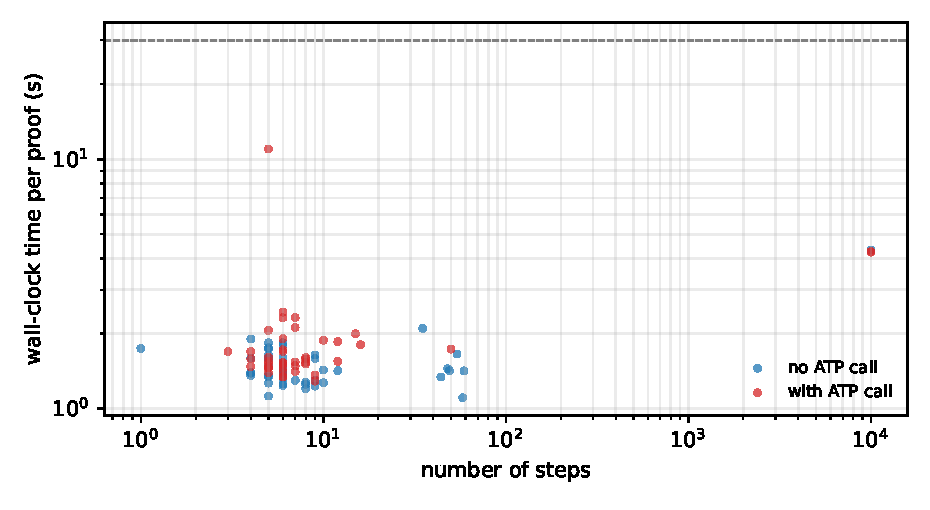
\includegraphics[width=\linewidth]{diagrams/runtime_scatter.pdf}
[Placeholder: wall-clock time per proof against the number of steps]
\caption{Wall-clock time per proof of the ProoVer set against the number of steps.}
\label{fig:eval-runtime}
\end{figure}

We also report where the time goes for the slowest proofs: parsing (LALR parser and transformer), global checks, rule checks, and ATP calls, and the peak memory of the worker process ([MB], measured with [tool]).
Deeply nested stress tests such as \texttt{PRV042} show whether the larger stack of Section~\ref{subsec:impl-resources} suffices: [result].

\subsection{Robustness (RQ3)}
\label{subsec:eval-robustness}

Robustness is evaluated in three ways.
First, the mutation test generates variants of valid seed proofs by applying one mutation each, such as changing a connective, swapping quantifiers, renaming a Skolem symbol to an existing one, or deleting a premise (Table~\ref{tab:eval-mutations}); a mutant is \emph{killed} if the verifier does not accept it.
Second, syntactically broken inputs (truncated files, unknown rules, missing annotations, deeply nested formulas) must neither crash the verifier nor lead to acceptance; we report the outcome for each class.
Third, we repeat the ProoVer run with the external prover removed from the path.
With the fail-closed policy, the number of wrong acceptances must stay at zero; the number of verified proofs drops by the proofs that need the ATP, and these proofs become uncertain.
This experiment verifies NFR1 empirically.

\begin{table}[t]
\centering
\small
\caption{Mutation operators and kill rates.}
\label{tab:eval-mutations}
\begin{tabular}{@{}l r r r@{}}
\toprule
Mutation operator & Mutants & Killed & Kill rate \\
\midrule
Change connective & [ ] & [ ] & [ ]\,\% \\
Swap quantifier kind & [ ] & [ ] & [ ]\,\% \\
Reuse existing symbol as Skolem symbol & [ ] & [ ] & [ ]\,\% \\
Remove premise & [ ] & [ ] & [ ]\,\% \\
\dots & & & \\
\midrule
Total & [ ] & [ ] & [ ]\,\% \\
\bottomrule
\end{tabular}
\end{table}

\subsection{Ablations}
\label{subsec:eval-ablation}

Two ablations quantify the design decisions of Table~\ref{tab:design-decisions}.
\emph{Syntactic checks first:} we run the verifier with all rule checkers disabled, so that every step goes to the external prover, and compare score and run time.
This shows what the internal checkers buy: [time factor] and [difference in score].
\emph{Three-valued verdict:} we replace the verdict rule by a binary one, in which unresolved steps count as failures, and recompute the score; the difference [D] shows the value of abstaining as described in Section~\ref{subsec:req-scoring}.
% Optional: Parser-Ablation (LALR vs. Earley) nur, falls ein Earley-Baseline noch existiert.

\subsection{Error Analysis}
\label{subsec:eval-errors}

We classify every proof of the ProoVer set whose verdict differs from the best possible one (acceptance of a valid proof, rejection of an invalid one) by its cause.
Table~\ref{tab:eval-errors} counts them by category: unsupported or imprecisely checked rule, missing ATP result, timeout, parser limitation, and expected result uncertain.
% TODO: pro Kategorie 1--2 konkrete Beispiele (Schrittname, Regel, Grund); bei Rewrite explizit auf die bekannte Lücke eingehen (Discussion).

\begin{table}[t]
\centering
\small
\caption{Causes of suboptimal verdicts on the ProoVer set.}
\label{tab:eval-errors}
\begin{tabular}{@{}l r l@{}}
\toprule
Cause & Proofs & Example \\
\midrule
Rule not checked precisely (e.g.\ \texttt{rewrite}) & [ ] & [ ] \\
ATP unresolved (timeout, no status) & [ ] & [ ] \\
Time limit exceeded & [ ] & [ ] \\
Parser or normalization limitation & [ ] & [ ] \\
\bottomrule
\end{tabular}
\end{table}

\subsection{Threats to Validity}
\label{subsec:eval-threats}

\paragraph{Internal validity.}
The verifier was developed against the ProoVer 2026 sample proofs, so the ProoVer set is not an independent test set; the TST set was written by the author and reflects the author's understanding of the rules.
The expected results of the ProoVer set depend on [source].
We mitigate this by reporting the mutation experiments, which do not depend on the benchmark, and by separating the wrong acceptances from the other errors.

\paragraph{External validity.}
The benchmark contains FOF proofs from a fixed set of generators; the results do not transfer to proofs from other provers with different rule vocabularies or to other logics.
The scoring scheme and the 30\,s limit are those of one competition.

\paragraph{Construct validity.}
The correctness of the accepted proofs relies on the correctness of the rule checkers, which is supported by tests but not proved, and on the soundness of the external prover.
Run times depend on the hardware and on the prover version and are therefore reported with their environment and as medians over several runs.

\subsection{Summary}
\label{subsec:eval-summary}

[TODO: three to five sentences answering RQ1--RQ3 with the key numbers; the full answers follow in Chapter~\ref{sec:conclusion}.]